\documentclass[10pt]{article}
\usepackage[ngerman]{babel}
\usepackage[utf8]{inputenc}
\usepackage[T1]{fontenc}
\usepackage{amsmath}
\usepackage{amsfonts}
\usepackage{amssymb}
\usepackage[version=4]{mhchem}
\usepackage{stmaryrd}
\usepackage{graphicx}
\usepackage[export]{adjustbox}
\graphicspath{ {./images/} }
\usepackage{mathtools}

\DeclareUnicodeCharacter{0131}{\ifmmode\imath\else{$\imath$}\fi}

\begin{document}
\section*{Zufallsstichproben}
\section*{Definition}
Eine einfache Zufallsstichprobe vom Umfang $n$ ist eine Folge von stochastisch unabhängigen und identisch verteilten Zufallsvariablen $X_{1}, \ldots, X_{n}$, den sogenannten Stichprobenvariablen. Dabei bezeichnet $X_{i}$ die Merkmalsausprägung des $i$-ten Elements in der Stichprobe. Die beobachteten Merkmalswerte $x_{1}, \ldots, x_{n}$ der $n$ Elemente sind Realisierungen der Zufallsvariablen $X_{1}, \ldots, X_{n}$ und heissen Stichprobenwerte.

\section*{Parameterschätzungen}
\section*{Definition}
Allgemein ist eine Stichprobenfunktion eine Funktion, die von den Stichprobenvariablen $X_{1}, \ldots, X_{n}$ abhängt. Eine Schätzfunktion $\Theta=g\left(X_{1}, \ldots, X_{n}\right)$ ist eine spezielle Stichprobenfunktion, nämlich eine „Formel", mit der man den Wert eines Parameters $\theta$ der Grundgesamtheit schätzen kann: Setzt man eine konkrete Stichprobe $x_{1}, \ldots x_{n}$ ein, so erhält man einen Schätzwert $\hat{\theta}=g\left(x_{1}, \ldots, x_{n}\right)$ für den Parameter $\theta$.

\section*{Definition}
Eine Schätzfunktion $\Theta$ eines Parameters $\theta$ heisst erwartungstreu, wenn gilt:

$$
E(\Theta)=\theta
$$

Gegeben sind zwei erwartungstreue Schätzfunktionen $\Theta_{1}$ und $\Theta_{2}$ desselben Parameters $\theta$. Man nennt $\Theta_{1}$ effizienter als $\Theta_{2}$, falls gilt:

$$
V\left(\Theta_{1}\right)<V\left(\Theta_{2}\right)
$$

Eine Schätzfunktion $\Theta$ eines Parameters $\theta$ heisst konsistent, wenn gilt:

$$
E(\Theta) \rightarrow \theta \text { und } V(\Theta) \rightarrow 0 \text { für } n \rightarrow \infty
$$

\section*{Schätzfunktionen für die wichtigsten statistischen Parameter}
\begin{center}
\begin{tabular}{|l|c|c|}
\hline
 & Schätzfunktion & Schätzwert \\
\hline
\begin{tabular}{l}
Erwartungswert \\
Spezialfall: Anteilswert \\
einer Bernoulli- \\
Verteilung \\
\end{tabular} & $\bar{X}=\frac{1}{n} \cdot \sum_{i=1}^{n} X_{i}$ & $\hat{p}=\bar{x}=\frac{1}{n} \sum_{i=1}^{n} x_{i}=\frac{\text { Anzahl len }}{n}$ \\
\hline
Varianz & $S^{2}=\frac{1}{n-1} \cdot \sum_{i=1}^{n}\left(X_{i}-\bar{X}\right)^{2}$ & $\hat{\sigma}^{2}=s^{2}=\frac{1}{n-1} \cdot \sum_{i=1}^{n}\left(x_{i}-\bar{x}\right)^{2}$ \\
\hline
Standardabweichung & $S=\sqrt{S^{2}}$ & $\hat{\sigma}=s=\sqrt{\frac{1}{n-1} \cdot \sum_{i=1}^{n}\left(x_{i}-\bar{x}\right)^{2}}$ \\
\hline
\end{tabular}
\end{center}

\section*{Satz}
(1) $\bar{X}$ und $S^{2}$ sind erwartungstreu und konsistent.\\
(2) $S$ ist konsistent, aber nicht erwartungstreu.

\section*{Vertrauensintervalle}
Man bestimmt zwei Stichprobenfunktionen $\Theta_{u}$ und $\Theta_{o}$, die den wahren Wert des Parameters $\theta$ mit der vorgegebenen Wahrscheinlichkeit $\gamma$ einschliessen:

$$
P\left(\Theta_{u} \leq \theta \leq \Theta_{o}\right)=\gamma
$$

Setzt man nun die Werte $x_{1}, x_{2}, \ldots, x_{n}$ einer konkreten Stichprobe in $\Theta_{u}$ und $\Theta_{o}$ ein, so erhält man die Zahlen $c_{u}$ und $c_{o}$. Das Intervall $\left[c_{u} ; c_{o}\right]$ ist dann ein Vertrauensintervall für den unbekannten Parameter $\theta$.

Die Wahrscheinlichkeit $\gamma$ heisst Vertrauensniveau oder statistische Sicherheit (übliche Werte: 95\% oder 99\%); $\alpha=1-\gamma$ wird Irrtumswahrscheinlı $\stackrel{\rightharpoonup}{1}$ genannt.

Wenn man hundertmal eine Stichprobe nehmen und zu jeder Stichprobe das Vertrauensintervall berechnen würde, so würden etwa $100 \cdot \gamma$ dieser Intervalle (bei $\gamma=95 \%$ also etwa 95) den wahren Wert des Parameters einschliessen:

\section*{Hundert 95\%-Vertrauensintervalle}
 Stichprobengrösse $\mathbf{n = 1 0}$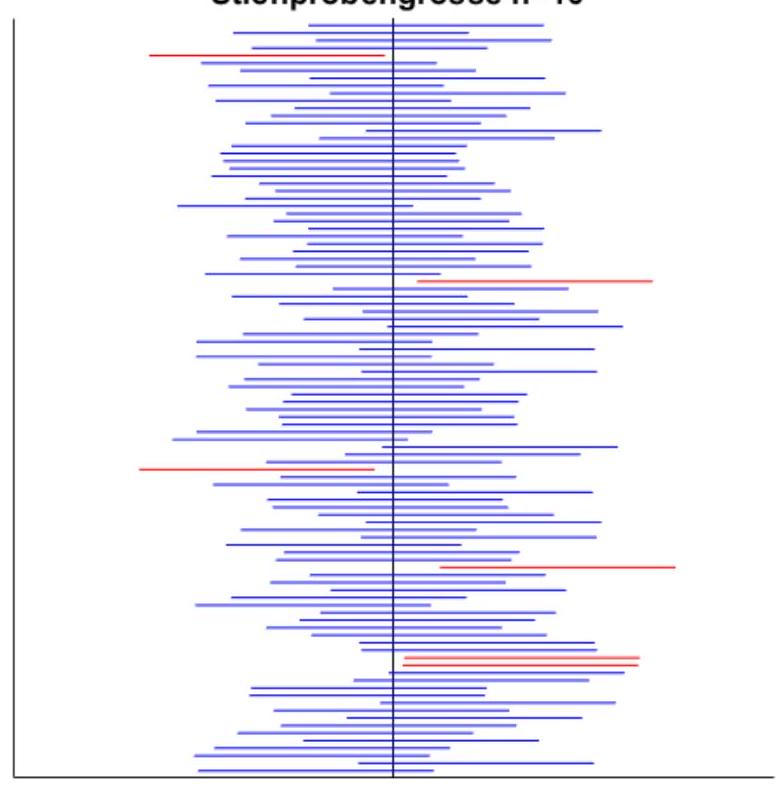
\includegraphics[width=\linewidth]{images/2025_01_02_5f577a434b389b742430g-2(1)}\\
wahrer Wert von $\theta$ (unbekannt)\\
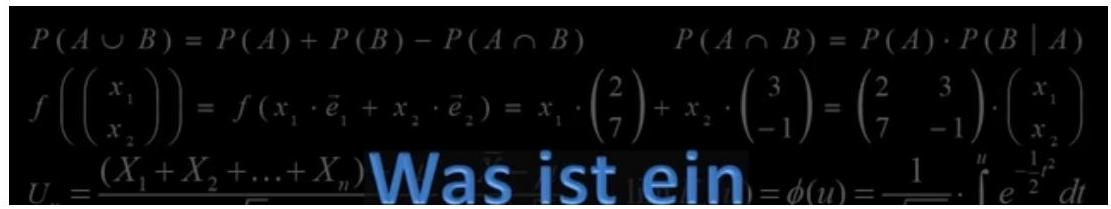
\includegraphics[width=\linewidth]{images/2025_01_02_5f577a434b389b742430g-2}\\
$>$ (1) 0:00 /8:04 $\qquad$

Übersicht über verschiedene Vertrauensintervalle zum Niveau $\gamma$

Tabular parse error: Open and close tags mismatch!,\\
\textbackslash begin\{tabular\}\{|c|c|c|c|c|c|c|\}
\textbackslash hline \& (1) Verteilung der Grundgesamtheit \& \textbackslash begin\{tabular\}\{l\}
(2) zu \textbackslash \textbackslash 
schätzender \textbackslash \textbackslash 
Parameter
\textbackslash end\{tabular\} \& (3) Schätzfunktionen \& (4) zugehörige standardisierte Zufallsvariable \& (5) Verteilung und benötigte Quantile \& \textbackslash begin\{tabular\}\{l\}
(6) Zufallsvariablen \textbackslash \textbackslash 
für Intervallgrenzen
\textbackslash end\{tabular\} \textbackslash \textbackslash 
\textbackslash hline 1 \& Normalverteilung (Varianz \$\textbackslash sigma\^{}\{2\}\$ bekannt) \& \$\textbackslash mu\$ \& \$\textbackslash bar\{X\}=\textbackslash frac\{1\}\{n\} \textbackslash cdot \textbackslash sum\_\{i=1\}\^{}\{n\} X\_\{i\}\$ \& \$U=\textbackslash frac\{\textbackslash bar\{X\}-\textbackslash mu\}\{\textbackslash sigma / \textbackslash sqrt\{n\}\}\$ \& \textbackslash begin\{tabular\}\{l\}
Standardnormalverteilung \textbackslash \textbackslash 
(Tabelle 2)
\$\$
c=u\_\{p\} \textbackslash text \{ mit \} p=\textbackslash frac\{1+\textbackslash gamma\}\{2\}
\$\$

\textbackslash end\{tabular\} \& \$\$

\[
\begin{aligned}
& \Theta_{u}=\bar{X}-c \cdot \frac{\sigma}{\sqrt{n}} \\
& \Theta_{o}=\bar{X}+c \cdot \stackrel{\varrho}{\Pi}
\end{aligned}
\]

\$\$ \\
\\
\textbackslash hline\\
\textbackslash end\{tabular\}

\textbackslash begin\{tabular\}\{|c|c|c|c|c|c|c|\}

\textbackslash hline 2 \& Normalverteilung (Varianz $\sigma^{2}$ unbekannt und $n \leq 30$; sonst Fall 1 mit $s$ als Schätzwert für $\sigma$ ) \& $\mu$ \& $$
\begin{gathered}
\bar{X}=\frac{1}{n} \cdot \sum_{i=1}^{n} X_{i} \\
S^{2}=\frac{1}{n-1} \cdot \sum_{i=1}^{n}\left(X_{i}-\bar{X}\right)^{2}
\end{gathered}
$$ \& $T=\frac{\bar{X}-\mu}{S / \sqrt{n}}$ \& $t$-Verteilung (Tabelle 4) mit $f=n-1$

$$
c=t_{(p ; f)} \text { mit } p=\frac{1+\gamma}{2}
$$ \& \$\$

\[
\begin{aligned}
\Theta_{u} & =\bar{X}-c \cdot S / \sqrt{n} \\
\Theta_{o} & =\bar{X}+c \cdot S / \sqrt{n}
\end{aligned}
\]

\$\$ \\


\textbackslash hline 3 \& Normalverteilung \& $\sigma^{2}$ \& \$\$\\
\[
\begin{gathered}
\bar{X}=\frac{1}{n} \cdot \sum_{i=1}^{n} X_{i} \\
S^{2}=\frac{1}{n-1} \cdot \sum_{i=1}^{n}\left(X_{i}-\bar{X}\right)^{2}
\end{gathered}
\]

$$ & $Z=(n-1) \frac{S^{2}}{\sigma^{2}}$ & \begin{tabular}{l}
Chi-Quadrat-Verteilung \\
(Tabelle 3) mit $f=n-1$
$$

\[
\begin{aligned}
& c_{1}=z_{\left(p_{1} ; f\right)} \text { mit } p_{1}=\frac{1-\gamma}{2} \\
& c_{2}=z_{\left(p_{2} ; f\right)} \text { mit } p_{2}=\frac{1+\gamma}{2}
\end{aligned}
\]

\$\$

\textbackslash end\{tabular\} \& \$\$

\[
\begin{aligned}
& \Theta_{u}=\frac{(n-1) \cdot S^{2}}{c_{2}} \\
& \Theta_{o}=\frac{(n-1) \cdot S^{2}}{c_{1}}
\end{aligned}
\]

$$ \\
\hline 4 & Bernoulli-Verteilung mit
$$

n \textbackslash hat\{p\}(1-\textbackslash hat\{p\})>9

\$\$ \& $p$ \& \textbackslash begin\{tabular\}\{l\}

$$
\bar{X}=\frac{1}{n} \cdot \sum_{i=1}^{n} X_{i}
$$

\\
\\
$X_{i}$ 0/1-wertig mit

$$
P\left(X_{i}=1\right)=p
$$

\textbackslash end\{tabular\} \& $U=\frac{\bar{X}-p}{\sqrt{p(1-p) / n}}$ \& Standardnormalverteilung näherungsweise (Tabelle 2)

$$
c=u_{q} \operatorname{mit} q=\frac{1+\gamma}{2}
$$ \& \$\$

\[
\begin{aligned}
& \Theta_{u}=\bar{X}-c \cdot \sqrt{\frac{\bar{X} \cdot(1-\bar{X})}{n}} \\
& \Theta_{o}=\bar{X}+c \cdot \sqrt{\frac{\bar{X} \cdot(1-\bar{X})}{n}}
\end{aligned}
\]

$$ \\
\hline 5 & beliebig mit
$$

n>30

\$\$ \& $\mu, \sigma^{2}$ \& wie im Fall \& (gegebenenfalls m \& $s$ als Schätzwert für $\sigma$ ) bzw. w \& im Fall 3 \\
\\
\textbackslash hline\\
\textbackslash end\{tabular\}

\section*{Hypothesentests}
\section*{Vorgehen bei einem Parametertest}
\section*{1. Nullhypothese $H_{0}$ aufstellen}
Um welchen Parameter geht es? Welchen Wert hat er angeblich? Oder werden zwei Parameter verglichen?

\section*{2. Alternativhypothese $H_{A}$ aufstellen}
Kommt es darauf an, in welche Richtung die Abweichung geht? Ist dies der Fall, so beschreibt $H_{A}$ nur die relevante Alternative.

\section*{3. Die richtige Zeile in der Tabelle "Übersicht über die wichtigsten Parametertests" finden}
Welcher Verteilung folgt die Grundgesamtheit? Um welche Nullhypothese geht es? Welcher Fall liegt vor?

\section*{4. Kritische Grenzen bestimmen}
Dabei müssen wir Folgendes berücksichtigen:

\begin{itemize}
  \item Verteilung der Testvariablen gemäss Tabelle "Übersicht über die wichtigsten Parametertests" (letzte Kolonne)
  \item Signifikanzniveau $\alpha$
  \item Ist $H_{A}$ einseitig oder zweiseitig? Wenn einseitig, auf welcher Seite befindet sich der kritische Bereich?
\end{itemize}

\section*{5. Testwert berechnen}
gemäss Tabelle "Übersicht über die wichtigsten Parametertests" (vorletzte Kolonne).

\section*{6. Testentscheidung fällen}
Liegt der Testwert im Annahmebereich oder im kritischen Bereich?

\section*{Übersicht über die wichtigsten Parametertests}
\begin{center}
\begin{tabular}{|c|c|c|c|c|c|c|}
\hline
 & \begin{tabular}{c}
Verteilung der \\
Grundgesamtheit \\
\end{tabular} & Nullhypothese & Fall & Schätzfunktion & \begin{tabular}{c}
Testvariable \\
(standardisiert) \\
\end{tabular} & \begin{tabular}{c}
Verteilung der \\
Testvariablen unter \\
$H_{0}$ \\
\end{tabular} \\
\hline
1 & Normalverteilung & $\mu=\mu_{0}$ & \begin{tabular}{c}
Varianz $\sigma^{2}$ bekannt \\
oder $n>30^{*}$ \\
\end{tabular} & $\bar{X}=\frac{1}{n} \cdot \sum_{i=1}^{n} X_{i}$ & $U=\frac{\bar{X}-\mu_{0}}{\sigma / \sqrt{n}}$ & \begin{tabular}{c}
Standardnormal- \\
verteilung (Tabelle 2) \\
\end{tabular} \\
\hline
2 & Normalverteilung & $\mu=\mu_{0}$ & \begin{tabular}{c}
Varianz $\sigma^{2}$ \\
unbekannt \\
\end{tabular} & $\bar{X}=\frac{1}{n} \cdot \sum_{i=1}^{n} X_{i}$ & $T=\frac{\bar{X}-\mu_{0}}{S / \sqrt{n}}$ & \begin{tabular}{c}
$t$-Verteilung mit \\
$f=n-1$ (Tabelle 4) \\
\end{tabular} \\
\hline
3 & \begin{tabular}{c}
Abhängige \\
2 Normal- \\
verteilungen \\
\end{tabular} & $\mu_{1}-\mu_{2}=0$ & \begin{tabular}{c}
Stichproben; \\
$\sigma_{2}^{2}$ bekannt oder \\
$n>30^{*}$ \\
\end{tabular} & $\bar{Z}=\bar{X}-\bar{Y}$ & \begin{tabular}{c}
$U=\frac{\bar{Z}}{\sigma}$ mit \\
$\sigma^{2}=\frac{\sigma_{1}^{2}+\sigma_{2}^{2}}{n}$ \\
\end{tabular} & \begin{tabular}{c}
Standardnormal- \\
verteilung (Tabelle 2) \\
\end{tabular} \\
\hline
\end{tabular}
\end{center}

\begin{center}
\begin{tabular}{|c|c|c|c|c|c|c|}
\hline
4 & 2 Normalverteilungen & $\mu_{1}-\mu_{2}=0$ & Abhängige Stichproben; Varianzen $\sigma_{1}^{2}$ und $\sigma_{2}^{2}$ unbekannt & \( \begin{gathered} \bar{Z}=\bar{X}-\bar{Y} \\ S^{2}=\frac{1}{n-1} \cdot \sum_{i=1}^{n}\left(X_{i}-Y_{i}-\bar{Z}\right)^{2} \end{gathered} \) & $T=\frac{\bar{Z}}{S / \sqrt{n}}$ & $t$-Verteilung mit $f=n-1$ (Tabelle 4) \\
\hline
5 & 2 Normalverteilungen & $\mu_{1}-\mu_{2}=0$ & Unabhängige Stichproben; Varianzen $\sigma_{1}^{2}$ und $\sigma_{2}^{2}$ bekannt oder $n_{1}, n_{2}>30^{*}$ & $\bar{Z}=\bar{X}-\bar{Y}$ & \( \begin{gathered} U=\frac{Z}{\sigma} \text { mit } \\ \sigma^{2}=\frac{\sigma_{1}^{1}}{n_{1}}+\frac{\sigma_{2}^{2}}{n_{2}} \end{gathered} \) & Standardnormalverteilung (Tabelle 2) \\
\hline
6 & 2 Normalverteilungen & $\mu_{1}-\mu_{2}=0$ & \begin{tabular}{l}
Unabhängige \\
Stichproben; \\
Varianzen $\sigma_{1}^{2}$ und $\sigma_{2}^{2}$ unbekannt, aber gleich \\
\end{tabular} & $T=\sqrt{\frac{n_{1} n_{2}\left(n_{1}+n_{2}-2\right)}{n_{1}+n_{2}}} \cdot \frac{}{\sqrt{\left(n_{1}-1\right)}}$ & $\frac{\bar{X}-\bar{Y}}{S_{1}^{2}+\left(n_{2}-1\right) S_{2}^{2}}$ & \begin{tabular}{l}
$t$-Verteilung mit \( f=n_{1}+n_{2}-2 \) \\
(Tabelle 4) \\
\end{tabular} \\
\hline
7 & Normalverteilung & $\sigma^{2}=\sigma_{0}^{2}$ &  & \( S^{2}=\frac{1}{n-1} \cdot \sum_{i=1}^{n}\left(X_{i}-\bar{X}\right)^{2} \) & $Z=(n-1) \frac{S^{2}}{\sigma_{0}^{2}}$ & Chi-Quadrat-Vert. mit $f=n-1$ (Tabelle 3) \\
\hline
8 & Bernoulli-Verteilung & $p=p_{0}$ &  & $\bar{X}=\frac{1}{n} \cdot \sum_{i=1}^{n} X_{i}=\frac{\text { Anzahl 1en }}{n}$ & $U=\frac{\bar{X}-p_{0}}{\sqrt{p_{0}\left(1-p_{0}\right) / n}}$ & \begin{tabular}{l}
näherungsweise \\
Standardnormal- \\
verteilung (Tabelle 2) \\
\end{tabular} \\
\hline
\end{tabular}
\end{center}

${ }^{*}$ ) Falls gilt: $n>30$ bzw. $n_{1}>30$ und $n_{2}>30$, so kann der entsprechende Fall für bekannte Varianzen angewendet werden; dabei dient $s$ als Schätzwert für $\sigma$ bzw. $s_{i}$ als Schätzwert für $\sigma_{i}$.

\section*{Mögliche Fehler bei einem Hypothesentest}
Bei einem Hypothesentest können zwei Arten von Fehlern auftreten:

\begin{center}
\begin{tabular}{|l|l|l|}
\hline
\multicolumn{1}{|c|}{\begin{tabular}{l}
Testentscheidung \\
Realität \\
\end{tabular}} & $H_{0}$ wird angenommen & $H_{0}$ wird abgelehnt \\
\hline
$H_{0}$ ist wahr &  & Fehler 1. Art \\
\hline
$H_{0}$ ist falsch & Fehler 2. Art &  \\
\hline
\end{tabular}
\end{center}

\section*{Der p-Wert}
Der p-Wert ist die Wahrscheinlichkeit, dass die Testvariable $T$ einen Wert annimmt, der mindestens so extrem ist wie der Testwert $\hat{t}$, der aufgrund der Stichprobe berechnet wurde, wenn $H_{0}$ wahr ist.\\
Die eingefärbte Fläche entspricht dem p-Wert\\
bei einer 2-seitigen Alternativhypothese

$H_{A}: \theta \neq \theta_{0}$.$\quad$\begin{tabular}{l}
Die eingefärbte Fläche entspricht dem p -Wert \\
bei einer 1-seitigen Alternativhypothese \\
$H_{A}: \theta>\theta_{0}$. \\
\end{tabular}

Zuletzt geändert: Samstag, 10. September 2022, 15:47

\section*{4 6. Zusammenfassung: Regression}

\end{document}